In this chapter, we consider the problem, which we refer to as \sigla{MCE}{Maximum Covering by Ellipses}. We introduce an algorithm for it, which in fact, works not only for ellipses but for any disk in a strictly convex normed plane.
\section{Definition}

Axis-parallel ellipses are defined as the set of points that satisfy \autoref{equation:pellipse}. All it takes to describe one is a pair of positive real numbers $(a,b) \in \R_{>0}^2$, with $a>b$, also called its shape parameters, and a center $q \in \R^2$.

An instance of MCE is given by a set of $n$ demand points $\Pp = \{p_1, \dots, p_n\}$, with $p_j\in\R^2$; 
a set of weights $\Ww:=\{w_1, \dots, w_n\}$, with $w_j\in\R_{\ge0}$ being the weight of point $p_j$;
and a set of $m$ axis-parallel ellipses given by their shape parameters $\Rr:=\{(a_1, b_1), \dots, (a_m, b_m)\}$, with $(a_j, b_j)\in\R_{>0}^2$ and $a_j>b_j$.
Additionally, to make the text more clear, we define a set $\E = \{E_1, \dots, E_m\}$, with $E_j : \R^2 \mapsto \R^2$ being a function that takes the center where the $j$-th ellipse is located as input, and returns its coverage region as defined by \autoref{equation:cover_pellipse}.

A solution for MCE is given by $Q:=(q_1, \dots, q_m)\in\R^{2m}$, with $q_j$ being the center of $j$-th ellipse.  Let $w: 2^{\Pp} \mapsto \R_{\ge0}$ be a function, which takes a subset of $\Pp$ and returns the sum of the weights of every point in it, defined as
\begin{equation*}
w(A) = \sum_{j : p_j \in A} w_j,
\end{equation*}
then an optimal solution of MCE is given by the optimization problem
\begin{equation*}
	\max_q w\left(\bigcup_{j=1}^m \Pp \cap E_j(q_j)\right).
\end{equation*}

\section{Related work}
The maximal planar covering using axis-parallel ellipses was first introduced in \citeonline{canbolat} which proposed a mixed integer non-linear programming method for the problem. This first approach showed to be not that efficient as it could not find an optimal solution for some instances within a timeout defined by them. To obtain solutions, not necessarily optimal ones, for the instances which the exact method showed inefficiency, a heuristic technique called Simulated Annealing was used to develop another method. Comparisons were made, which showed that the second approach was able to obtain good solutions, compared to the optimal ones found for some of the instances, within a good run-time.

The second work found in the literature was \citeonline{andreta}, which developed a method that breaks the problem into smaller ones fixing the set of points an ellipse is going to cover. For each set of points fixed as the points an ellipse is going to cover, a small optimization problem is solved to find out if there is a location where the ellipse can be placed, so to cover the set of fixed points. To enumerate the possible solutions and then find an optimal one, the method defined a data structure that stores every set of points an ellipse can cover. This method showed better results and was able to find optimal solutions for the instances that the first method could not get as well as for new created instances.

\subsection{Maximum cover by disks}
In \citeonline{cabello:2006}, a $\bigO(n^{2m-1}\log{n})$ algorithm for $MCD$ is developed as a sub-routine for its $(1-\epsilon)$-approximation algorithm. Firstly, they solve a sub-problem for two disks in $\bigO(n^3\log{n})$. Then, for the rest of the points that are not in that solution, it uses the algorithm developed in \citeonline{chazelle:1986} for the one-disk case, checking every possible solution for every one of the disks left.

Also, in \citeonline{zhou} an heuristic method for large-scale $MCD$ is proposed. It uses a probabilistic algorithm called mean-shift which is a gradient ascent method proven to converge to a local density maxima of any probability distribution. The mean-shift is utilized to find good candidates of centers for the unit disks, then the method backtracks to find the best assignment. The results showed that the greedy algorithm achieves an optimal coverage in some instances, but for some other ones it has a 15 percent worse coverage ratio.

Two exact methods for the case of MCD with only one disk have been found in the literature. A $\bigO(n^2)$ algorithm is proposed by \citeonline{chazelle:1986} which improved the previously $\bigO(n^2\log{n})$ one proposed by \citeonline{drezner}.
As it has been mentioned, MCD for one disk is a 3SUM-HARD problem, which means that it is as hard as the 3SUM problem (the problem of finding three real numbers that sum to zero, given $n$ real numbers). Initially the lower bound of the 3SUM problem was conjectured to be $\Omega(n^2)$, matching the best algorithm for MCD for one disk, which meant that no better time-complexity could be achieved. Since then, however, better algorithms for 3SUM have been developed with a $\bigO(\frac{n^2}{poly(n)})$ run time complexity \cite{3SUM-kopelowitz:2014}.

In \citeonline{drezner}, the main idea used to develop the $\bigO(n^2\log{n})$ algorithm is that, even though there are infinitely many points where the disk could be placed, only a few of them, a finite amount of $\bigO(n^2)$, needs to be considered for the method to find an optimal solution.
The algorithm, for every point, sorts the other points with respect to the angle they form with the first one. After that, the first point is placed on the border of the disk and, going through the sorted list, the algorithm inserts and removes points from the disk coverage. Also, when inserting and removing a point from the coverage, it only checks the disk centers that make the entering/leaving point to be on the border. Because the algorithm only checks the centers that make the disk have two points on its border, the number of centers it goes through is bounded by the number of pairs of points, which is $\binom{n}{2} = \bigO(n^2)$.

\section{Strictly Convex Normed Plane}

In this section, we give a brief introduction to the notion of strictly convex normed planes, which is utilized in the rest of the chapter.

Given a vector space $\mathscr{V}$, and a norm function $||\cdot|| \colon \mathscr{V} \to \R_{\ge0}$ for that vector space, we denote by $(\mathscr{V}, ||\cdot||)$ the normed vector space with respect to $\mathscr{V}$ and $||\cdot||$.
A strictly convex normed space is defined in \citeonline{wada} as a normed vector space whose every chord of its unit sphere has its midpoint in the interior of its unit ball. In other words, in a strictly convex normed space, no line intersects a unit sphere more than twice. 
We also refer to norms that induce strictly convex normed spaces as strictly convex norms.
Restricting this definition to $\R^2$, we get a strictly convex normed plane, and we refer to its ball as disk, and to its sphere as circle.
For more details about convexity and strictly convexity see \citeonline{conv}.

For example, the norms $||x||_p=(\sum_{i} |x_i|^p)^{\frac{1}{p}}$, $p\in \mathbb{N}, p>1$ define strictly convex unit disks, while $||\cdot||_1$ and $||\cdot||_{\infty}$ do not.
Given the shape parameters $(a, b)$ of an ellipse, it is possible to define a strictly convex normed space $(\R^2,||\cdot||_{a,b})$, such that the unit circle $\{x \in \R^2\colon ||x||_{a, b} = 1\}$ is the axis-parallel ellipse with shape parameters $(a, b)$ centered at the origin.

Instead of developing an algorithm for ellipses only, based on the results of \citeonline{bi}, we describe a more general method that only assumes that the facilities have a strictly convex coverage area, and it is possible to determine the intersection between the boundaries of two of them.
We refer to this more general version of MCE as \sigla{MCSCD}{Planar Maximum Covering Location by Strictly Convex Disks}, and instead of having a list of shape parameters, a list of strictly convex norm functions $\F=\{f_1, \dots, f_m\}$ is given, and an instance of MCSCD is defined as the tuple $(\Pp, \Ww, \F)$. Also, we define for MCSCD the set $\E=\{E_1, \dots, E_m\}$, with $E_j\colon \R^2 \to \R^2$ being a function that takes a center where the $j$-th disk is located and returns the unit disk corresponding to the the norm $f_i$.

\section{Maximum Weight Clique}

We introduce in this section a problem which is equivalent to the version of MCSCD with only one facility. We refer to this equivalent problem as \sigla{MWC}{Maximum Weight Clique}. This equivalence is also used in the works for MCD in \citeonline{chazelle:1986} and \citeonline{cabello:2006}. Later we use the developments for this problem to construct a CLS for each disk in an instance of MCSCD.

An instance of the \sigla{MWC}{Maximum Weight Clique} is given by a list of points \mbox{$\Pp:=\{p_1,\dots,p_n\}$}, with $p_i \in \R^2$; 
a norm $||\cdot||$, such that $(\R^2, ||\cdot||)$ is a strictly convex normed plane; and a set of weights \mbox{$\Ww:=\{w_1, \dots, w_n\}$}, with $w_i\in \R_{>0}$. 
Then, we define a set of unit disks $\D:=\{D_1, \dots, D_n\}$, with $D_i:=\{x \in \R^2 \colon ||x-p_i|| \le 1\}$ being a unit disk centered at $p_i$; we also denote by $\partial D_i$ as the circle correspondent to the $i$-th unit disk, and that $w_i$ is the weight of $D_i$.
All that being said, we define an instance of MWC as a tuple $(\Pp, \Ww, ||\cdot||)$.

In this context, a clique is a non-empty intersection region of one or more disks. The weight of a clique is the sum of every disk's weight in it.
Following this, we define a solution for MWC as just a point $q\in\cup_{j=1}^n D_j$, which is inside any of the given disks in $\D$.
From a solution $q$, the corresponding clique $S$ can be obtained by intersecting every disk that contains $q$ as follows
\begin{equation*}
	S = \bigcap_{j : q \in D_j} D_j.
\end{equation*}
Therefore, an optimal solution of MWC is defined as	$\max_{q} \sum_{D_k \cap q \neq \emptyset} w_k$.


Let $D$ be a unit disk in a strictly convex normed plane $(\R^2, ||\cdot||)$, and $p, q \in \partial D$. Then we denote by $\widehat{p, q}$ as the counter-clockwise arc of $D$ starting at $p$ and ending at $q$. This is represented in \autoref{fig:disk_arc} where the arc $\widehat{p,q}$ is shown with a solid line, and the arc $\widehat{q, p}$ is shown by a dashed line.

\begin{figure}[!htb]
	\centering
	
	\caption{The definition of arcs of a circle.}
	%\usetikzlibrary{matrix}



\tikzset{every picture/.style={line width=0.75pt}} %set default line width to 0.75pt        

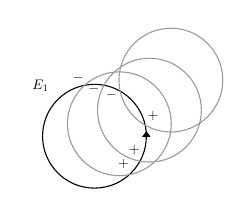
\begin{tikzpicture}[x=0.75pt,y=0.75pt,yscale=-1,xscale=1]
%uncomment if require: \path (0,95); %set diagram left start at 0, and has height of 95

%Shape: Circle [id:dp37777408295388804] 
\draw   (21,59.5) .. controls (21,45.69) and (32.19,34.5) .. (46,34.5) .. controls (59.81,34.5) and (71,45.69) .. (71,59.5) .. controls (71,73.31) and (59.81,84.5) .. (46,84.5) .. controls (32.19,84.5) and (21,73.31) .. (21,59.5) -- cycle ;
%Shape: Circle [id:dp4562198988843913] 
\draw  [color={rgb, 255:red, 155; green, 155; blue, 155 }  ,draw opacity=1 ] (47.5,46.94) .. controls (47.5,33.14) and (58.69,21.94) .. (72.5,21.94) .. controls (86.31,21.94) and (97.5,33.14) .. (97.5,46.94) .. controls (97.5,60.75) and (86.31,71.94) .. (72.5,71.94) .. controls (58.69,71.94) and (47.5,60.75) .. (47.5,46.94) -- cycle ;
%Shape: Circle [id:dp8913971633985722] 
\draw  [color={rgb, 255:red, 155; green, 155; blue, 155 }  ,draw opacity=1 ] (33,53.5) .. controls (33,39.69) and (44.19,28.5) .. (58,28.5) .. controls (71.81,28.5) and (83,39.69) .. (83,53.5) .. controls (83,67.31) and (71.81,78.5) .. (58,78.5) .. controls (44.19,78.5) and (33,67.31) .. (33,53.5) -- cycle ;
%Shape: Circle [id:dp05970043129919356] 
\draw  [color={rgb, 255:red, 155; green, 155; blue, 155 }  ,draw opacity=1 ] (57.81,32.47) .. controls (57.81,18.66) and (69,7.47) .. (82.81,7.47) .. controls (96.62,7.47) and (107.81,18.66) .. (107.81,32.47) .. controls (107.81,46.27) and (96.62,57.47) .. (82.81,57.47) .. controls (69,57.47) and (57.81,46.27) .. (57.81,32.47) -- cycle ;
%Straight Lines [id:da04725899028195979] 
%\draw[densely dotted]  (21,59.5) -- (71,59.5) ;


%Flowchart: Extract [id:dp5267407418119328] 
\draw  [fill={rgb, 255:red, 0; green, 0; blue, 0 }  ,fill opacity=1 ] (71,57.45) -- (72.52,59.55) -- (69.48,59.55) -- cycle ;

\draw (60,73) node [scale=0.5]  {$+$};
% Text Node
\draw (65.22,66) node [scale=0.5]  {$+$};
% Text Node
\draw (74.22,50) node [scale=0.5]  {$+$};
% Text Node
\draw (54.22,39.56) node [scale=0.5]  {$-$};
% Text Node
\draw (45.62,36.96) node [scale=0.5]  {$-$};
% Text Node
\draw (38.02,31.56) node [scale=0.5]  {$-$};


% Text Node
\draw (20,35) node [scale=0.5]  {$E_{1}$};
\end{tikzpicture}

\begin{tikzpicture}

\matrix [matrix of nodes,row sep=,row sep=0mm,
column 1/.style={nodes={rectangle,draw,minimum width=1.5em, minimum height=0.5em}},
column 2/.style={nodes={rectangle,draw,minimum width=1.5em, minimum height=0.5em}},
column 3/.style={nodes={rectangle,draw,minimum width=1.5em, minimum height=0.5em}},
column 4/.style={nodes={rectangle,draw,minimum width=1.5em, minimum height=0.5em}},
column 5/.style={nodes={rectangle,draw,minimum width=1.5em, minimum height=0.5em}},
column 6/.style={nodes={rectangle,draw,minimum width=1.5em, minimum height=0.5em}},
column 7/.style={nodes={rectangle,draw,minimum width=1.5em, color=gray, minimum height=0.5em}},
column 8/.style={nodes={rectangle,draw,minimum width=1.5em, color=gray, minimum height=0.5em}},
column 9/.style={nodes={rectangle,draw,minimum width=1.5em, color=gray, minimum height=0.5em}},
column 10/.style={nodes={rectangle,draw,minimum width=1.5em, color=gray, minimum height=0.5em}},
column 11/.style={nodes={rectangle,draw,minimum width=1.5em, color=gray, minimum height=0.5em}},
column 12/.style={nodes={rectangle,draw,minimum width=1.5em, color=gray, minimum height=0.5em}}
] (O)
{
$+$ & $-$ & $-$ & $-$ & $+$ & $+$ & $+$ & $-$ & $-$ & $-$ & $+$ & $+$\\
%$+$ & $-$ & $-$ & $-$ & $+$ & $+$\\
};

\node at (-4,-0.5) {$0$};
\node at (0,-0.5) {$2\pi$};
\end{tikzpicture}
	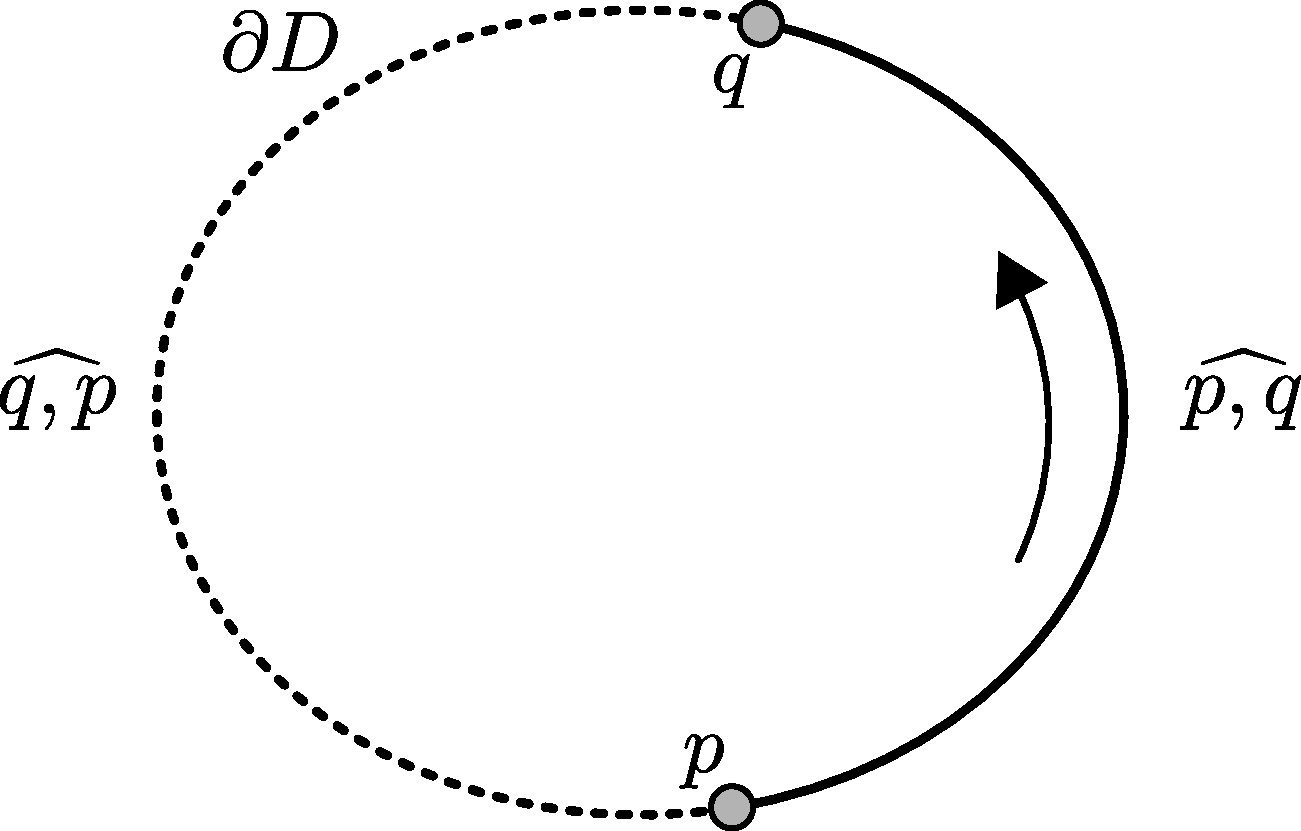
\includegraphics[scale=.3]{tex/figures/disk_arc.pdf}
	\fautor
	\label{fig:disk_arc}
\end{figure}

Let $(\Pp, \Ww, \{||\cdot||\})$ be an instance of MCSCD with only one facility, and $(\Pp, \Ww, ||\cdot||)$ an instance of MWC.
If $q_1$ be a solution for the MCSCD's instance. Then, the disks with centers in $\Pp \cap E_1(q_1)$ have a non-empty intersection.
Also, suppose that $q$ is a solution of MWC. Then, the ellipse with shape parameters $(a, b)$ centered at $q$ covers the points, which are the centers of disks, such that $q \in D_j$.
Therefore, MCSCD and MWC for both problems are equivalent.

Let us consider the intersection set of $k$ unit disks $\cap_{j=1}^k D_j(x_j)$, for any strictly convex normed space, with $x_j \in \R^2$, $j\in \{1, \dots, k\}$ being all distinct.
Then, in \citeonline{bi}, the following results are stated about that set: its boundary is formed by arcs of unit circles whose centers are in $\{x_1, \dots, x_k\}$, its vertices are in the set $\partial D_i(x_i) \cap \partial D_j(x_j)$, for any $i \neq j$; and $|\partial D_i(x_i) \cap \partial D_j(x_j)| \le 2$, for any $i\neq j$. 
Based on that, we introduce the next definition.

\begin{definicao}
	Let $D_i$ and $D_j$ be two unit disk in a strictly convex normed space, and\\ \mbox{$\{\alpha_{ij}^+, \alpha_{ij}^-\} = \partial D_i(p_i) \cap \partial D_j(p_j)$},
	 we denote by $\widehat{\alpha_{ij}^+, \alpha_{ij}^-}$ the minimal counter-clockwise arc of $\partial D_i$ starting in $\alpha_{ij}^+$ and ending in $\alpha_{ij}^-$. We also refer to $\alpha_{ij}^+$ as an opening intersection point, and to $\alpha_{ij}^-$ as a closing intersection point.
	 If $\partial D_i$ and $\partial D_j$ intersect at exactly one point, we define $\alpha_{ij}^+ = \alpha_{ij}^- = \partial D_i \cap \partial D_j$.
\end{definicao}
Let $\widehat{\alpha_{ij}^+, \alpha_{ij}^-}$ and $\widehat{\alpha_{ij}^-, \alpha_{ij}^+}$ be the two arcs of $\partial D_i$ with respect to the endpoints $\alpha_{ij}^-, \alpha_{ij}^+$.
From \citeonline[Lemma 2]{bi}, we can state that, $\widehat{\alpha_{ij}^+, \alpha_{ij}^-}\subset D_j$, and\\ $\widehat{\alpha_{ij}^-, \alpha_{ij}^+} \cap D_j = \{\alpha_{ij}^-, \alpha_{ij}^+\}$. That is, only the minimal arc is contained in the interior of $D_j$. In \autoref{fig:disk_arc_inter}, the minimal arcs are highlighted with a solid border, and it is possible to see that they are the only ones that are in the intersection's interior.

\begin{figure}[!htb]
	\centering
	
	\caption{The intersection between two circles, and the arcs .}
	%\usetikzlibrary{matrix}



\tikzset{every picture/.style={line width=0.75pt}} %set default line width to 0.75pt        

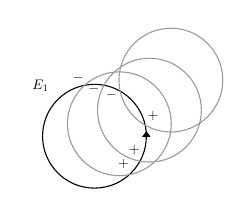
\begin{tikzpicture}[x=0.75pt,y=0.75pt,yscale=-1,xscale=1]
%uncomment if require: \path (0,95); %set diagram left start at 0, and has height of 95

%Shape: Circle [id:dp37777408295388804] 
\draw   (21,59.5) .. controls (21,45.69) and (32.19,34.5) .. (46,34.5) .. controls (59.81,34.5) and (71,45.69) .. (71,59.5) .. controls (71,73.31) and (59.81,84.5) .. (46,84.5) .. controls (32.19,84.5) and (21,73.31) .. (21,59.5) -- cycle ;
%Shape: Circle [id:dp4562198988843913] 
\draw  [color={rgb, 255:red, 155; green, 155; blue, 155 }  ,draw opacity=1 ] (47.5,46.94) .. controls (47.5,33.14) and (58.69,21.94) .. (72.5,21.94) .. controls (86.31,21.94) and (97.5,33.14) .. (97.5,46.94) .. controls (97.5,60.75) and (86.31,71.94) .. (72.5,71.94) .. controls (58.69,71.94) and (47.5,60.75) .. (47.5,46.94) -- cycle ;
%Shape: Circle [id:dp8913971633985722] 
\draw  [color={rgb, 255:red, 155; green, 155; blue, 155 }  ,draw opacity=1 ] (33,53.5) .. controls (33,39.69) and (44.19,28.5) .. (58,28.5) .. controls (71.81,28.5) and (83,39.69) .. (83,53.5) .. controls (83,67.31) and (71.81,78.5) .. (58,78.5) .. controls (44.19,78.5) and (33,67.31) .. (33,53.5) -- cycle ;
%Shape: Circle [id:dp05970043129919356] 
\draw  [color={rgb, 255:red, 155; green, 155; blue, 155 }  ,draw opacity=1 ] (57.81,32.47) .. controls (57.81,18.66) and (69,7.47) .. (82.81,7.47) .. controls (96.62,7.47) and (107.81,18.66) .. (107.81,32.47) .. controls (107.81,46.27) and (96.62,57.47) .. (82.81,57.47) .. controls (69,57.47) and (57.81,46.27) .. (57.81,32.47) -- cycle ;
%Straight Lines [id:da04725899028195979] 
%\draw[densely dotted]  (21,59.5) -- (71,59.5) ;


%Flowchart: Extract [id:dp5267407418119328] 
\draw  [fill={rgb, 255:red, 0; green, 0; blue, 0 }  ,fill opacity=1 ] (71,57.45) -- (72.52,59.55) -- (69.48,59.55) -- cycle ;

\draw (60,73) node [scale=0.5]  {$+$};
% Text Node
\draw (65.22,66) node [scale=0.5]  {$+$};
% Text Node
\draw (74.22,50) node [scale=0.5]  {$+$};
% Text Node
\draw (54.22,39.56) node [scale=0.5]  {$-$};
% Text Node
\draw (45.62,36.96) node [scale=0.5]  {$-$};
% Text Node
\draw (38.02,31.56) node [scale=0.5]  {$-$};


% Text Node
\draw (20,35) node [scale=0.5]  {$E_{1}$};
\end{tikzpicture}

\begin{tikzpicture}

\matrix [matrix of nodes,row sep=,row sep=0mm,
column 1/.style={nodes={rectangle,draw,minimum width=1.5em, minimum height=0.5em}},
column 2/.style={nodes={rectangle,draw,minimum width=1.5em, minimum height=0.5em}},
column 3/.style={nodes={rectangle,draw,minimum width=1.5em, minimum height=0.5em}},
column 4/.style={nodes={rectangle,draw,minimum width=1.5em, minimum height=0.5em}},
column 5/.style={nodes={rectangle,draw,minimum width=1.5em, minimum height=0.5em}},
column 6/.style={nodes={rectangle,draw,minimum width=1.5em, minimum height=0.5em}},
column 7/.style={nodes={rectangle,draw,minimum width=1.5em, color=gray, minimum height=0.5em}},
column 8/.style={nodes={rectangle,draw,minimum width=1.5em, color=gray, minimum height=0.5em}},
column 9/.style={nodes={rectangle,draw,minimum width=1.5em, color=gray, minimum height=0.5em}},
column 10/.style={nodes={rectangle,draw,minimum width=1.5em, color=gray, minimum height=0.5em}},
column 11/.style={nodes={rectangle,draw,minimum width=1.5em, color=gray, minimum height=0.5em}},
column 12/.style={nodes={rectangle,draw,minimum width=1.5em, color=gray, minimum height=0.5em}}
] (O)
{
$+$ & $-$ & $-$ & $-$ & $+$ & $+$ & $+$ & $-$ & $-$ & $-$ & $+$ & $+$\\
%$+$ & $-$ & $-$ & $-$ & $+$ & $+$\\
};

\node at (-4,-0.5) {$0$};
\node at (0,-0.5) {$2\pi$};
\end{tikzpicture}
	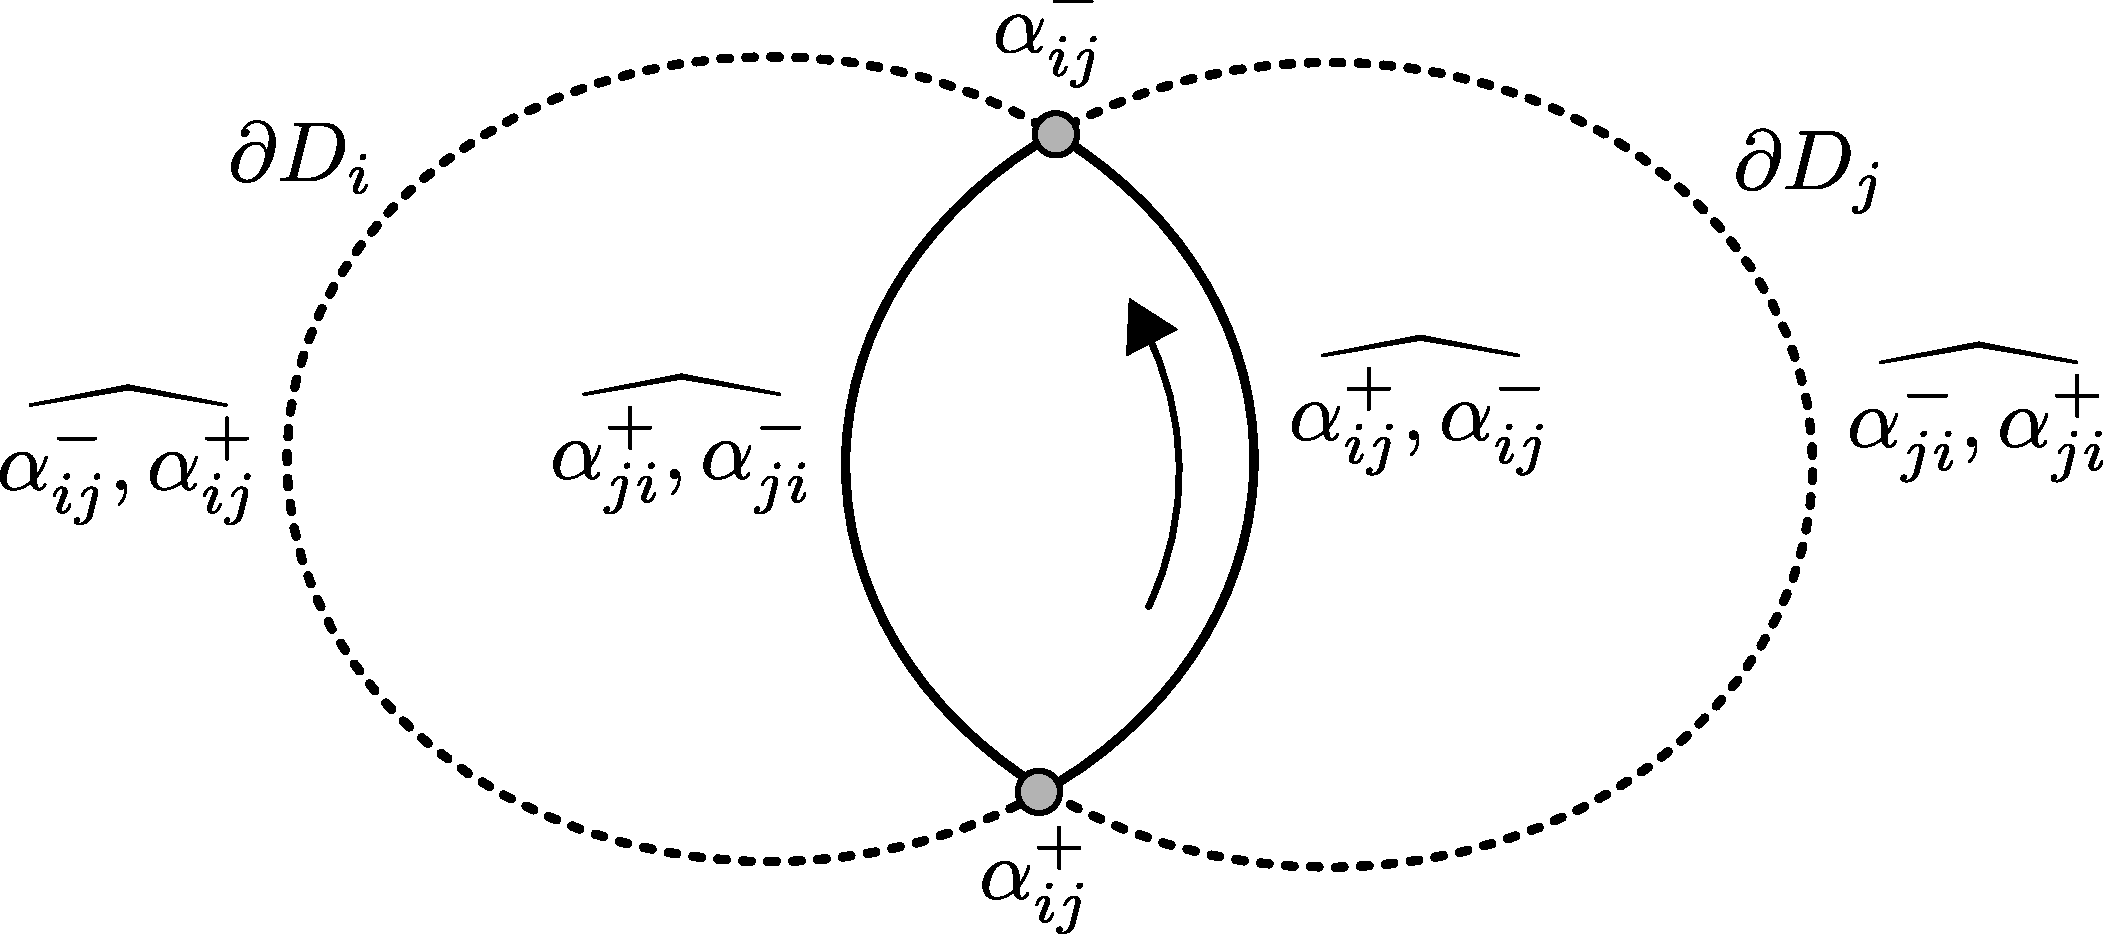
\includegraphics[scale=.3]{tex/figures/disk_arc_inter.pdf}
	\fautor
	\label{fig:disk_arc_inter}
\end{figure}


Based on that, we are going to develop an algorithm that finds the best clique that $\partial D_i$ is part of, for each $i=1, \dots, n$, and then combine the solutions to get an overall optimal one. Notice that this is enough because, by \citeonline{bi}, the arcs of the circles in $\partial \D$ form the boundary of any clique.
For each $i\in \{1, \dots, m\}$, let $q_i$ be an optimal solution of MWC with an additional constraint that $q_i \in \partial D_i$.
Then, an optimal solution of MWC can be obtained by just taking a solution of
$\max_{i=1}^n \max_{q \in \partial D_i} \sum_{D_k \cap q} w_k$.

\begin{lema}\label{lema:mwc}
	Let $(\Pp, \Ww, ||\cdot||)$ be an instance of MWC. For each $i\in \{1, \dots, n\}$,
	let $q_i$ be any solution, such that $q_i \in \partial D_i$; and $J=\{j \colon q_i \in D_j\}$. If there is \mbox{$j \in \{1, \dots, n\}$}, $j\neq i$, such that $D_i \cap D_j \neq \emptyset$, then $q_i \in \cap_{j \in J, j\neq i}\{\widehat{\alpha_{ij}^+, \alpha_{ij}^-}\}$.
\end{lema}

\begin{proof}
	Suppose that $q_i \not \in \widehat{\alpha_{ij}^+, \alpha_{ij}^-}$, for some $j \in J\setminus \{i\}$.
	By definition $q_i \in \partial D_i$, and by \citeonline[Lemma 2]{bi}, we have that $q_i \in \widehat{\alpha_{ij}^-, \alpha_{ij}^+}$, which implies that $q_i \in \{\alpha_{ij}^-, \alpha_{ij}^+\}$, which would imply that  $q_i \in \widehat{\alpha_{ij}^+, \alpha_{ij}^-}$, contradicting the assumption we made.
\end{proof}

Given the set of indexes $J=\{j \colon q_i \in D_j\}$ of disks that contain a solution $q_i\in\partial D_i$, we have that there exists $l, k \in J\setminus \{i\}$, such that  $\cap_{j \in J, j\neq i}\{\widehat{\alpha_{ij}^+, \alpha_{ij}^-}\} = \widehat{\alpha_{il}^+, \alpha_{ik}^-}$. Therefore, by \autoref{lema:mwc}, we can just look for an index $l \in \{1, \dots, n\} \setminus \{i\}$, such that it is the solution of $$\max_{l \neq i} \sum_{D_k \cap \alpha_{il}^+} w_k.$$ 
Then an optimal solution $q_i \in \partial D_i$ can be obtained by just setting $q_i = \alpha_{il}^+$. From that, a $\bigO(n^3)$ algorithm for MWC can be developed by just evaluating, for every pair $i, j \in \{1, \dots, n\}$, the solution defined by $\alpha_{ij}^+$. 
Based on the algorithms for MCD proposed by \citeonline{drezner} and \citeonline{cabello:2006} though, we can develop a $\bigO(n^2\lg{n})$ algorithm for MWC.
Let $A_i$ be a circular defined as 
\begin{equation*}
	A_i = \{\alpha_{ij}^+ \colon j\neq i, D_i \cap D_j \neq \emptyset\} \cup \{\alpha_{ij}^- \colon j\neq i, D_i \cap D_j \neq \emptyset \},
\end{equation*}
which contains all the intersection points of $\partial D_i$ with all the other disks. Assume that this list is sorted by the angles on $D_i$ in the interval $[0, 2\pi)$ corresponding to the intersection points, breaking ties prioritizing opening intersection points. 
Finding the best solution which $D_i$ is part of can be done by traversing $A_i$ while keeping a set of active disks. When an opening intersection angle is reached, the corresponding disk is added to the active set; and when a closing one is seen, the corresponding disk is removed from the active set. This way, finding an optimal solution can be achieved by keeping the weight of the active disks as well as the best clique found so far.

In practice, traversing a circular list can be emulated by traversing a regular list that has a copy of the original circular list added to its end. 
Therefore, the list $B_i$ is defined here as a list that contains the elements of $A_i$, and a copy of it shifted to the interval $[2\pi, 4\pi]$. It is defined as
\begin{equation}\label{eq:bi2}
B_i = A_i\cup\bigcup_{j\neq i} \{2\pi+\alpha_{ij}^+ \colon j\neq i, D_i \cap D_j \neq \emptyset\} \cup \{2\pi+\alpha_{ij}^- \colon j\neq i, D_i \cap D_j \neq \emptyset \}.
\end{equation}
Assuming $B_i$ is sorted with the same criteria as $A_i$, a simple traversal, starting at the first element and going until the last one, simulates a traversal on the circular list $A_i$.
This works because for any pair of disks $D_i$, $D_j$; $B_i$ contains $\alpha_{ij}^+ < \alpha_{ij}^- + 2\pi$. That is, the algorithm encounters an opening intersection point before reaching a closing one for any circle.

If it is possible to find the intersection between two unit disks (it will be shown that it is possible for the case where the unit disk is an axis-parallel ellipse), for each disk, the runtime complexity of processing every intersection point and sorting the list $B_i$ is $\bigO(n\lg{n})$. Therefore, the overall runtime complexity of this algorithm for MWC is $\bigO(n^2\lg{n})$.

In \autoref{fig:array_disks2}, the intersection points between $\partial D_1$ (solid border) with $\partial D_2, \partial D_3$, and $\partial D_4$ (dashed border) are shown with a plus or minus sign indicating opening or closing intersection points. 
The intersection list $B_1$ is also displayed in \autoref{fig:array_disks2} along with the size of the set of active disks $Q$ after processing a point in $B_1$.
It is possible to see that the optimal clique highlighted in \autoref{fig:array_disks2} is enclosed by the arcs defined by $\alpha_{14}^+$ and $\alpha_{14}^-$, and can also be identified by following $B_1$ while keeping track of $Q$.
The special intersection point of $\partial D_1$ with itself can also be seen in \autoref{fig:array_disks2}. Its usage is very convenient as with $\alpha_{11}^+$ and $\alpha_{11}^-$  in $B_1$, the algorithm inserts $D_1$ in the set of active disks before processing any point, and removes $D_1$ only after every point has been processed.

\begin{figure}[!htb]
	\centering
	
	\caption{The intersection list of a disk with three other disks.}
	%\usetikzlibrary{matrix}



\tikzset{every picture/.style={line width=0.75pt}} %set default line width to 0.75pt        

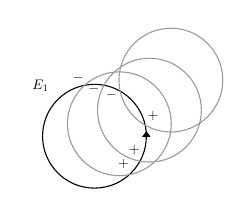
\begin{tikzpicture}[x=0.75pt,y=0.75pt,yscale=-1,xscale=1]
%uncomment if require: \path (0,95); %set diagram left start at 0, and has height of 95

%Shape: Circle [id:dp37777408295388804] 
\draw   (21,59.5) .. controls (21,45.69) and (32.19,34.5) .. (46,34.5) .. controls (59.81,34.5) and (71,45.69) .. (71,59.5) .. controls (71,73.31) and (59.81,84.5) .. (46,84.5) .. controls (32.19,84.5) and (21,73.31) .. (21,59.5) -- cycle ;
%Shape: Circle [id:dp4562198988843913] 
\draw  [color={rgb, 255:red, 155; green, 155; blue, 155 }  ,draw opacity=1 ] (47.5,46.94) .. controls (47.5,33.14) and (58.69,21.94) .. (72.5,21.94) .. controls (86.31,21.94) and (97.5,33.14) .. (97.5,46.94) .. controls (97.5,60.75) and (86.31,71.94) .. (72.5,71.94) .. controls (58.69,71.94) and (47.5,60.75) .. (47.5,46.94) -- cycle ;
%Shape: Circle [id:dp8913971633985722] 
\draw  [color={rgb, 255:red, 155; green, 155; blue, 155 }  ,draw opacity=1 ] (33,53.5) .. controls (33,39.69) and (44.19,28.5) .. (58,28.5) .. controls (71.81,28.5) and (83,39.69) .. (83,53.5) .. controls (83,67.31) and (71.81,78.5) .. (58,78.5) .. controls (44.19,78.5) and (33,67.31) .. (33,53.5) -- cycle ;
%Shape: Circle [id:dp05970043129919356] 
\draw  [color={rgb, 255:red, 155; green, 155; blue, 155 }  ,draw opacity=1 ] (57.81,32.47) .. controls (57.81,18.66) and (69,7.47) .. (82.81,7.47) .. controls (96.62,7.47) and (107.81,18.66) .. (107.81,32.47) .. controls (107.81,46.27) and (96.62,57.47) .. (82.81,57.47) .. controls (69,57.47) and (57.81,46.27) .. (57.81,32.47) -- cycle ;
%Straight Lines [id:da04725899028195979] 
%\draw[densely dotted]  (21,59.5) -- (71,59.5) ;


%Flowchart: Extract [id:dp5267407418119328] 
\draw  [fill={rgb, 255:red, 0; green, 0; blue, 0 }  ,fill opacity=1 ] (71,57.45) -- (72.52,59.55) -- (69.48,59.55) -- cycle ;

\draw (60,73) node [scale=0.5]  {$+$};
% Text Node
\draw (65.22,66) node [scale=0.5]  {$+$};
% Text Node
\draw (74.22,50) node [scale=0.5]  {$+$};
% Text Node
\draw (54.22,39.56) node [scale=0.5]  {$-$};
% Text Node
\draw (45.62,36.96) node [scale=0.5]  {$-$};
% Text Node
\draw (38.02,31.56) node [scale=0.5]  {$-$};


% Text Node
\draw (20,35) node [scale=0.5]  {$E_{1}$};
\end{tikzpicture}

\begin{tikzpicture}

\matrix [matrix of nodes,row sep=,row sep=0mm,
column 1/.style={nodes={rectangle,draw,minimum width=1.5em, minimum height=0.5em}},
column 2/.style={nodes={rectangle,draw,minimum width=1.5em, minimum height=0.5em}},
column 3/.style={nodes={rectangle,draw,minimum width=1.5em, minimum height=0.5em}},
column 4/.style={nodes={rectangle,draw,minimum width=1.5em, minimum height=0.5em}},
column 5/.style={nodes={rectangle,draw,minimum width=1.5em, minimum height=0.5em}},
column 6/.style={nodes={rectangle,draw,minimum width=1.5em, minimum height=0.5em}},
column 7/.style={nodes={rectangle,draw,minimum width=1.5em, color=gray, minimum height=0.5em}},
column 8/.style={nodes={rectangle,draw,minimum width=1.5em, color=gray, minimum height=0.5em}},
column 9/.style={nodes={rectangle,draw,minimum width=1.5em, color=gray, minimum height=0.5em}},
column 10/.style={nodes={rectangle,draw,minimum width=1.5em, color=gray, minimum height=0.5em}},
column 11/.style={nodes={rectangle,draw,minimum width=1.5em, color=gray, minimum height=0.5em}},
column 12/.style={nodes={rectangle,draw,minimum width=1.5em, color=gray, minimum height=0.5em}}
] (O)
{
$+$ & $-$ & $-$ & $-$ & $+$ & $+$ & $+$ & $-$ & $-$ & $-$ & $+$ & $+$\\
%$+$ & $-$ & $-$ & $-$ & $+$ & $+$\\
};

\node at (-4,-0.5) {$0$};
\node at (0,-0.5) {$2\pi$};
\end{tikzpicture}
	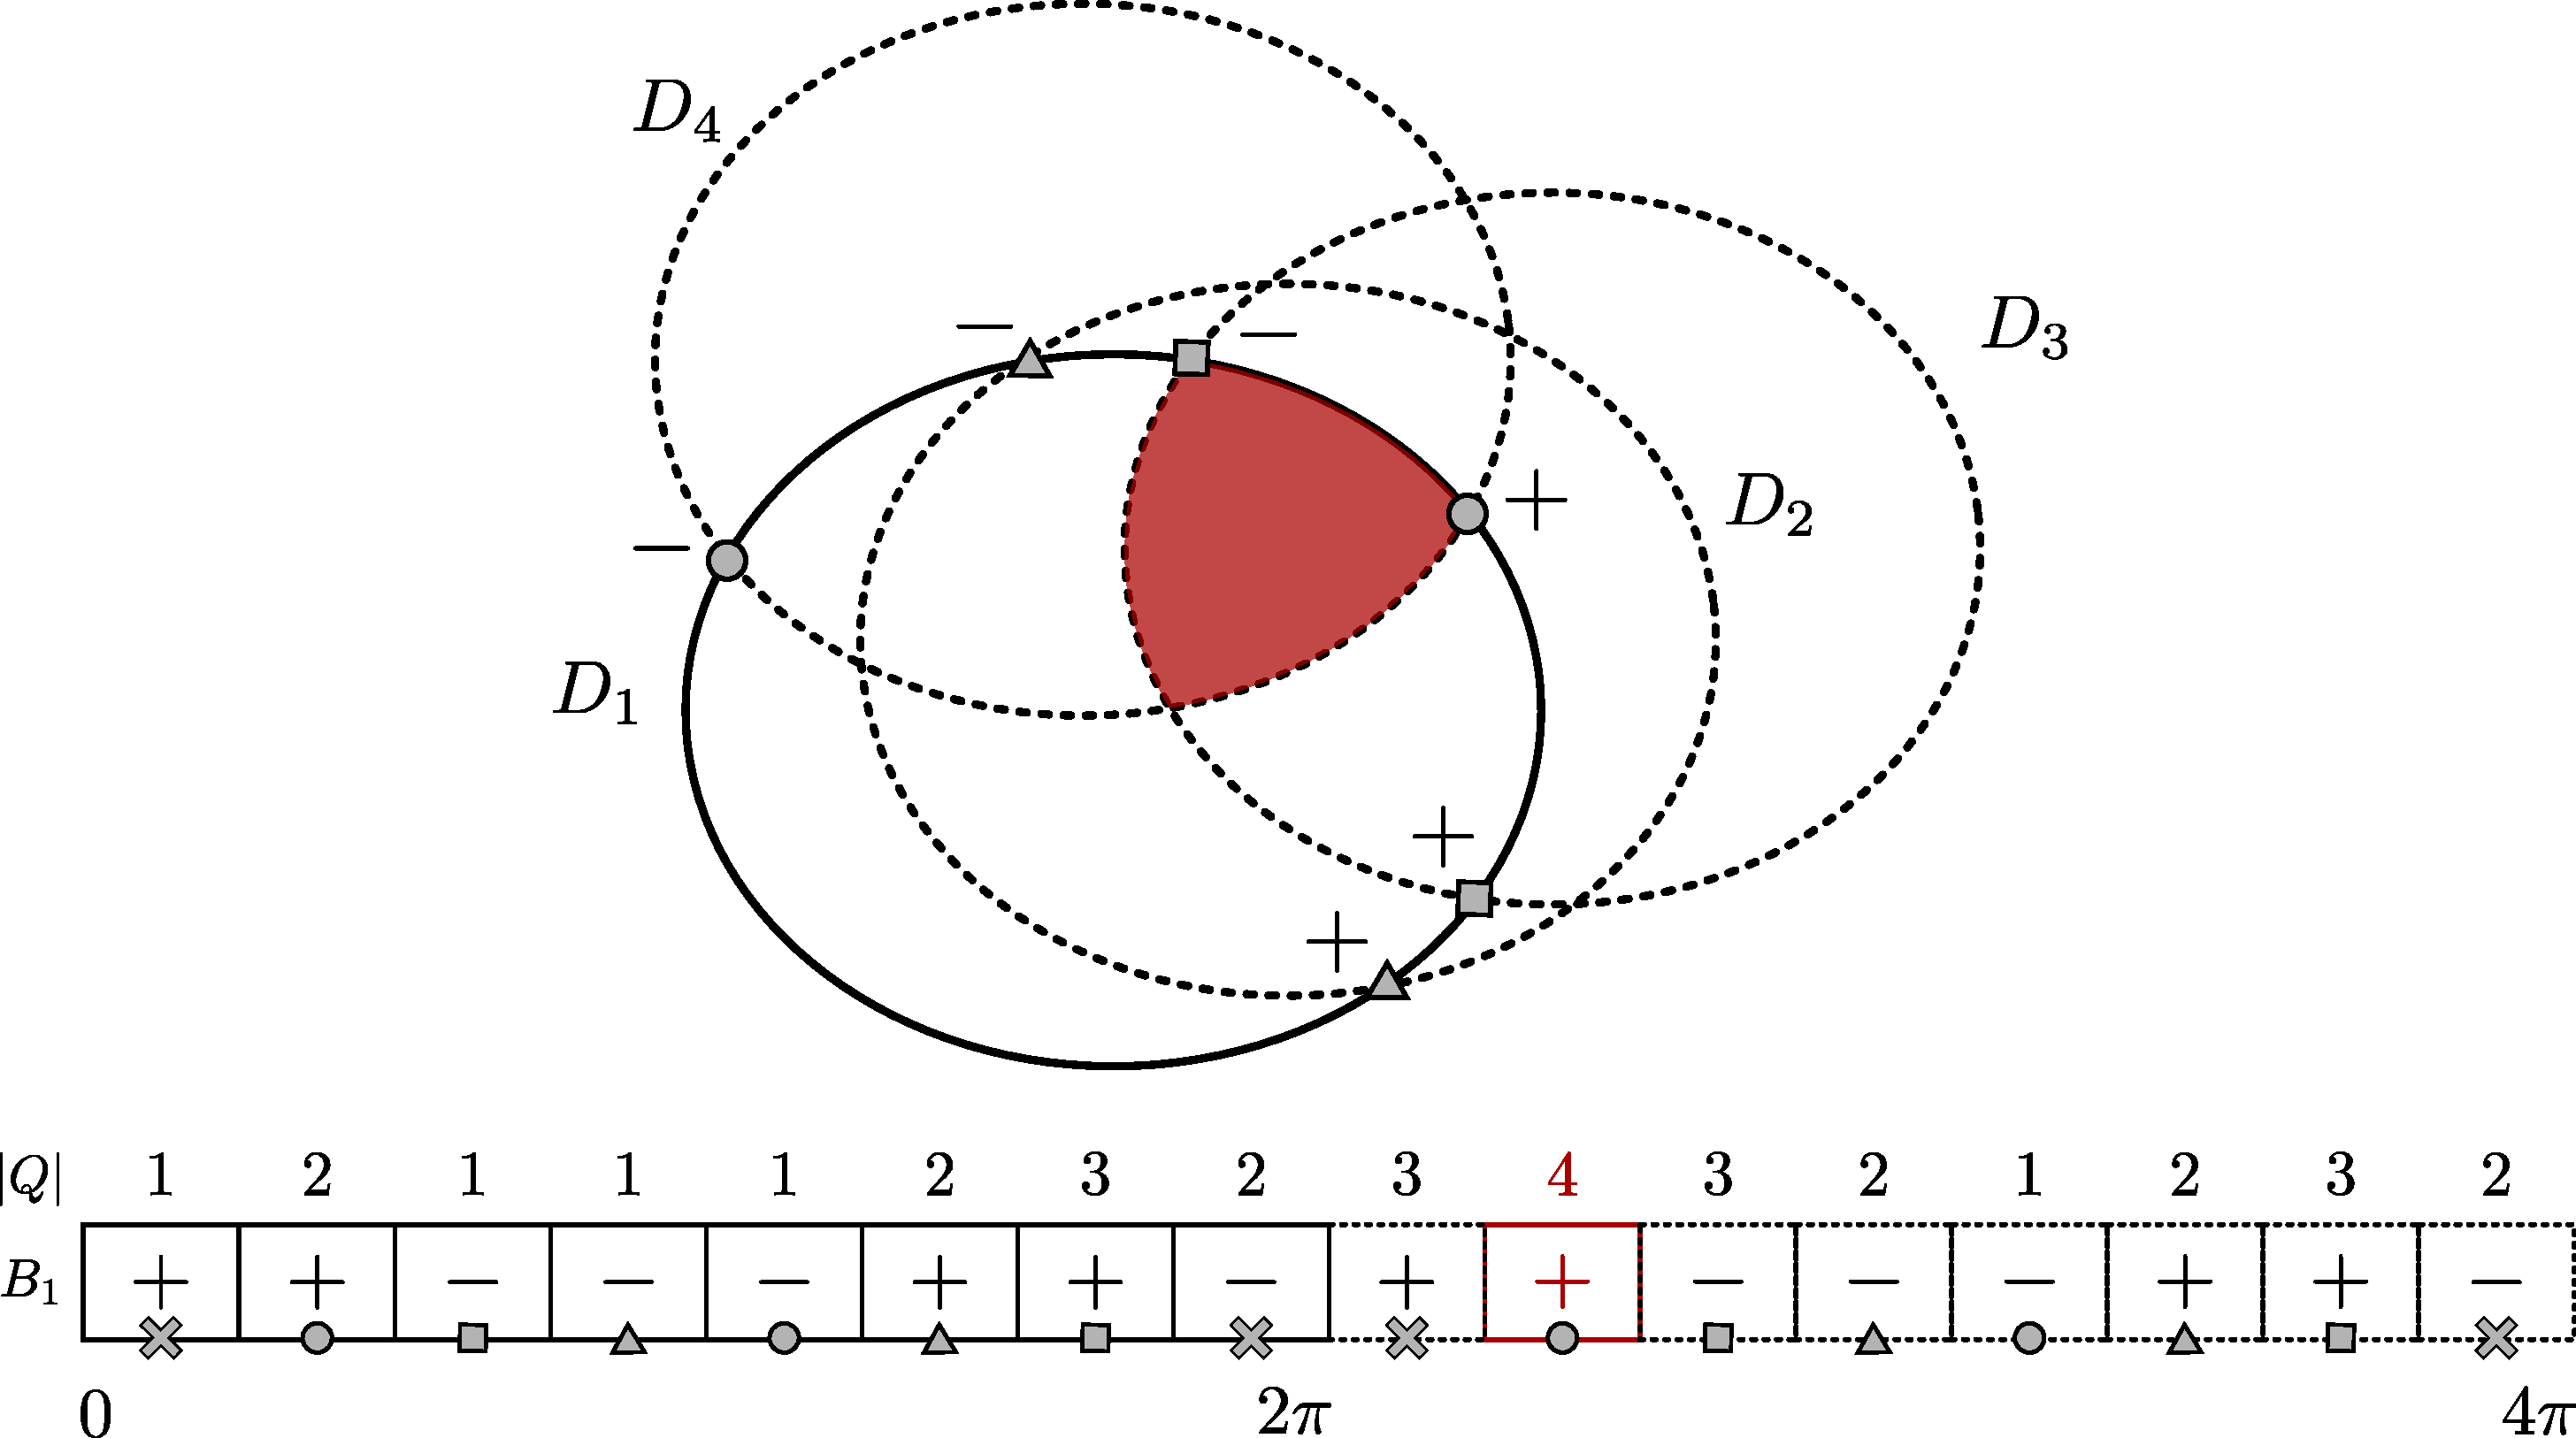
\includegraphics[scale=.3]{tex/figures/3_disks_intersect_.pdf}
	\fautor
	\label{fig:array_disks2}
\end{figure}

%\begin{algoritmo}[!htb]
%	\caption{Algorithm for MWC.}\label{algoritmo:mwc}
%	\begin{algorithmic}[1]
%		\Require{A set of points $\Pp=\{p_1,\dots,p_n\}$, and a set of weights $\Ww=\{w_1, \dots, w_n\}$.}
%		\Ensure{A point that is inside the maximum weight clique of unit disks.}
		
%		\item[]
		
%		\Procedure{$MWC$}{$\Pp, \Ww$}
%		\State Let $\D=\{D_1, \dots, D_n\}$ be a set of unit disks, with centers in $\Pp$ and weights in $\Ww$
		
%		\State $Q_{best} \gets \{\}$
%		\State $q^* \gets$ $p_1$
%		\ForAll{$D_i \in \D$}
%		\State Let $B_i$ be the list of intersection angles of $D_i$ as defined by \autoref{eq:b_i}
		
%		\State $Q \gets \{\}$ \Comment{The set of active disks.}
%		\For{$\alpha \in B_i$}\Comment{Assuming $B_i$ is sorted.}
%		\State Let $D_j$ be the disk, such that $\theta \in D_j\cap D_i$
%		\If{$\theta$ is a opening angle}
%		\State $Q \gets Q \cup \{D_j\}$
%		\Else
%		\State $Q \gets Q \setminus \{D_j\}$
%		\EndIf
%		\If{$w(Q_{best}) < w(Q)$} 
%		\State $Q_{best} \gets Q$
%		\State $q^* \gets$ point corresponding to the intersection angle $\theta$
%		\EndIf
%		
%		\EndFor
%		\EndFor
		
%		\State \Return $q^*$
%		\EndProcedure
%	\end{algorithmic}
%\end{algoritmo}

\section{From MWC to MCSCD}

Based on the ideas developed for MWC, we are going to propose an algorithm for MCSCD in this section assuming that for each $f_i \in \F$, it is possible to determine the intersection between two translated unit disks determined by $f_i$.
Then later, we give details of how to determine the intersection between two ellipses, and develop an algorithm for MCE.

Suppose that an instance $(\Pp, \Ww, \F)$ of MCSCD is given. For each $f_i \in \F$, we have the equivalent instance $(\Pp, \Ww, f_i)$ of MWC. Next, we introduce a definition for the CLS of each facility.

\begin{definicao}
	Let $(\Pp, \Ww, \F)$ be an instance of MCSCD. For each $j \in \{1, \dots, m\}$, let \mbox{$(\Pp,  \Ww, f_j)$} be the equivalent instance of MWC, we define as the \sigla{CLS}{Candidate List Set} $S_j$ for $j$-th facility as
	\begin{equation*}
	S_j = \bigcup_{i=1}^n \{\alpha_{ik}^+ \colon k\neq i, D_i \cap D_k \neq \emptyset\}\cup \{p_i\}.
	\end{equation*}
\end{definicao}

For each $f_j \in \F$, we consider every pairwise opening -- we could have chose the closing ones -- intersection between the circles induced by $f_j$ centered at every point in $\Pp$.
Based on this, we introduce a theorem that allows us to develop an algorithm for MCSCD based on the developments we made for MWC.

\begin{theorem}\label{th:mce2}
	Let $(\Pp, \Ww, \F)$ be an instance of MCSCD, and $\Omega(\Pp, \Ww, \F)$ be a set of solutions defined as 
	\begin{equation*}\label{eq:omega2}
		\Omega(\Pp, \Ww, \F) = \{Q\in \R^{2m} \colon q_j \in S_j \textnormal{ for all } j\in\{1, \dots, m\}\},
	\end{equation*}
	Then there exists an optimal solution $Q^*\in \Omega(\Pp, \Ww, \F)$, and $|\Omega(\Pp, \Ww, \F)|\le n^{2m}$.
\end{theorem}
\begin{proof}
		Notice that $\Omega(\Pp, \Ww, \F)$ is defined as the combination of every possible solution from each CLS. 
		To prove that $\Omega(\Pp, \Ww, \F)$ contains an optimal solution, we just need to show that for any optimal solution $Q'$, for every $j \in \{1, \dots, m\}$, there exists $q_j \in S_j$, such that $\Pp \cap E_j(q_j') \subset \Pp \cap E_j(q_j)$.
		That is, we only need to show that the CLS of every ellipse contains a center that makes the ellipse cover the same points (possibly some additional ones) that it covers in an optimal solution.
		We ignore the case where an ellipse does not cover any points.
		
		First case: $|\Pp \cap E_j(q_j')|=1$. This case is included in $S_j$ as it contains the possible solutions where the center of the ellipse is the actual points in $\Pp$.
		
		Second case: $|\Pp \cap E_j(q_j')| > 1$. Let $X = \{i \colon p_i \in \Pp \cap E_j(q_j')\}$. In the equivalent instance of MWC, we have that $\cap_{i\in X} D_i \neq \emptyset$ is a region bounded by arcs of circles with centers in $\Pp \cap E_j(q_j')$ with vertices being pairwise intersections of $\partial \D$. By \autoref{lema:mwc}, we have that at least one of the vertices of $\cap_{i\in X} D_i$ is an opening intersection point.
		
		Lastly, we have that $|S_j| \le \binom{n}{2} + n = \frac{n(n+1)}{2} \le n^2$. Therefore,
		$|\Omega(\Pp, \Ww, \F)| \le |S_1|\times \dots \times |S_m| \le n^{2m}$.
\end{proof}
%%%%

Based on \autoref{th:mce2}, we can define an algorithm to enumerate every solution in $\Omega(\Pp, \Ww, \F)$. If determining $\alpha_{ij}^+$ is possible for every $i, j \in \{1, \dots, n\}$, this algorithm can be implemented to have a $\bigO(mn^{2m+1})$ runtime complexity, if $\bigO(nm)$ operations is taken to evaluate each solution.
In the next section, we describe an algorithm for MCE, giving the details on how to determine the intersection between two ellipses.

\section{An algorithm for MCE}

Based on \autoref{th:mce2}, in \autoref{algoritmo:mce_cls} we define a simple $\bigO(n^2)$ procedure called CLS-MCE that returns a CLS given a set of points and an ellipse's shape parameters.
Then in \autoref{algoritmo:mce2}, we define another procedure which backtracks the CLS returned by \autoref{algoritmo:mce_cls} of every ellipse to find an optimal solution given an instance of MCE. This algorithm can be implemented to have a $\bigO(mn^{2m+1})$ runtime complexity if the CLSs are constructed beforehand in a preprocessing phase. 

%%%%%


\begin{algoritmo}
	\caption{Algorithm that returns a CLS for an ellipse.}\label{algoritmo:mce_cls}
	\begin{algorithmic}[1]
		\Require{A set of points $\Pp=\{p_1,\dots,p_n\}$ with weights $\Ww=\{w_1, \dots, w_n\}$, and an ellipse's shape parameters $(a, b)$.}
		\Ensure{A CLS for the given ellipse.}
		
		\item[]
		
		\Procedure{CLS-MCE}{$\Pp, \Ww, (a, b)$}
		\State Let $\D$ be a set of unit disks on the strictly convex normed space $(\R^2, ||.||_{a, b})$.
		\State $S \gets \{\}$
		\ForAll{$p_i \in \Pp$}
		\State $S \gets S \cup \{p_i\}$
		
		\ForAll{$j \neq i \colon D_j \cap D_i \neq \emptyset$}

		\State $S \gets S \cup \{\alpha_{ij}^+\}$	

		\EndFor
		\EndFor
		
		\State \Return $S$
		\EndProcedure
	\end{algorithmic}
\end{algoritmo}

\subsection{Determining $\alpha_{ij}^+$ and $\alpha_{ij}^-$ for axis-parallel ellipses}\label{section:ellipses_intersection2}

Let $E_1(q_1)$, and $E_2(q_2)$ be two coverage region of ellipses centered at $q_1, q_2\in\R^2$ respectively, with shape parameters $(a, b)\in\R^2_{>0}$. After changing the coordinates to make the center of the first ellipse be at the origin, the intersection points between the two ellipses are defined by

\begin{align}
	\frac{x^2}{a^2} + \frac{y^2}{b^2} = 1 && (E_1) \label{eq:ell_inter_1}\\
	\frac{(x-h)^2}{a^2} + \frac{(y-k)^2}{b^2} = 1 && (E_2), \nonumber
\end{align}
where $(h,k)\in\R^2$ is the center of the second ellipse after the coordinates were translated by $-q_1$. As both equations are equal to $1$, we have
\begin{align}
	b^2x^2 + a^2y^2 &= b^2(x-h)^2 + a^2(y-k)^2 \nonumber\\
	x &= y\frac{-2ka^2}{2hb^2} + \frac{b^2h^2 + a^2k^2}{2hb^2} \nonumber\\
	x &= y\alpha + \beta.\label{eq:ell_inter_2}
\end{align}
Replacing \autoref{eq:ell_inter_2} into \autoref{eq:ell_inter_1}, we get
\begin{align}\label{eq:ell_inter_3}
	y^2(b^2\alpha^2 + a^2) + y(2\beta\alpha b^2) + b^2\beta^2 -a^2b^2 = 0,
\end{align}
which is a second degree polynomial. Then, $\partial E_1(q_1) \cap \partial E_2(q_2) \neq \{\}$ if, and only if the roots of \autoref{eq:ell_inter_3} are real. The intersection points itself can be obtained by solving the polynomial for $y$ and plugging its value back into the $x=y\alpha + \beta$ equation.

Suppose that $\partial E_1(q_1) \cap \partial E_2(q_2) = \{p_1, p_2\}$, with $p_1 \neq p_2$. To determine $\alpha_{12}^+$ and $\alpha_{12}^-$, we need to first determine the intersection angles corresponding to $p_1$ and $p_2$ on $E_1(q_1)$. 

Let $\gamma_1$ and $\gamma_2$ be two curves defined as \autoref{eq:parametric_ellipse} for $E_1(q_1)$ and $E_2(q_2)$ respectively. 
The intersection angle of $p_i$ in $E_j(q_j)$ is defined as $t_i^{(j)} \in [0, 2\pi)$, such that $\gamma_j(t_i^{(j)}) = p_i$, for $i, j \in \{1, 2\}$. Obtaining $t_i^{(j)}$ can be done analytically solving the equation

\begin{equation}\label{eq:angle_inter}
	\dfrac{a}{b}\dfrac{p_{iy}-q_{jy}}{p_{ix}-q_{jx}} = \tan{(t_i^{(j)})}.
\end{equation}

Determining which one of the points is $\alpha_{ij}^+$, we just need to use the assumption that $\widehat{\alpha_{ij}^+, \alpha_{ij}^-}$ is minimal. This can be done using the angle of the intersection points obtained from \autoref{eq:angle_inter}. 

\begin{algoritmo}
	\caption{Algorithm for MCE}\label{algoritmo:mce2}
	
	\begin{algorithmic}[1]
		\Require{A set of points $\Pp=\{p_1,\dots,p_n\}$, a list of weights $\Ww=\{w_1, \dots, w_n\}$, and a list of shape parameters $\Rr=\{(a_1, b_1), \dots, (a_m, b_m)\}$.}
		
		\Ensure{An optimal solution for MCE.}
		
		\item[]
		\Procedure{$MCE$}{$\Pp, \Ww, \Rr$}
		\State \Return $MCE_{bt}(\Pp, \Ww, \Rr, 1)$
		\EndProcedure
		\State
		\Procedure{$MCE_{bt}$}{$Z, \Ww, \Rr, j$}
		\If{$j = m+1$}
		\State \Return $0$
		\EndIf
		
		\State $(q_j^*, \dots, q_m^*) \gets (0, \dots, 0)$
		
		\State $S_j \gets \textnormal{CLS-MCE}(Z, a_j, b_j)$
		\For{$q_j \in S_j$}
		\State $Cov \gets \Pp \cap E_j(q_j)$
		\State $(q_{j+1}, \dots, q_m) \gets MCE_{bt}(Z \setminus Cov, \Ww, \Rr, j+1)\}$
		
		\If{$w(\cup_{k=j}^m Z \cap E_k(q_k)) >  w(\cup_{k=j}^m Z \cap E_k(q_k^*))$}
		\State $(q_j^*, \dots, q_m^*) \gets(q_j, \dots, q_m)$
		\EndIf
		\EndFor
		
		\State \Return $(q_j^*, \dots, q_m^*)$
		\EndProcedure
	\end{algorithmic}
\end{algoritmo}


\section{Adding facility cost}

Additionally, in \citeonline{andreta} and \citeonline{canbolat}, two other parameters are present in the definition of the problem. This extension is the result of having costs associated with every facility.
In MCE, though, the total cost, which is the sum of costs of every used facility, is constant; hence, to create a decision about which ones are utilized, a new parameter $k\in\mathbb{N}$ is given, along with a constraint on the number of used ellipses.

We refer to this version of the problem as  \sigla{MCE-$k$}{Planar Maximum Covering Location by Ellipses with a $k$-constraint}. An instance of it is given by the same parameters as MCE, plus a list of costs $\Cc=\{c_1, \dots, c_m\}$, with $c_j\in\R_{\ge0}$ being the $j$-th ellipse's cost, and $k\in\mathbb{N}$, $k\le m$.

A solution for MCE-$k$, however,  when compared to MCE's, has a bit more cluttered description. We define it as a set $I:=\{i_1, \dots, i_k\}\subset\{1, \dots, m\}$, such that $|I|=k$; and a tuple $Q:=(q_1, \dots, q_k)$, with $q_j\in\R^2$ being the center of the $j$-th ellipse in $I$. An optimal solution of MCE-$k$ is given by the optimization problem

\begin{equation*}
	\max_{I, Q} w\left(\bigcup_{j=1}^k \Pp \cap E_{i_j}(q_j)\right).
\end{equation*}

Finally, \autoref{algoritmo:mce2} can serve as basis for MCE-$k$'s \autoref{algoritmo:mce-k}. 
Firstly, for every subset $I \subset \{1, \dots, m\}$, such that $|I| = k$, the algorithm for MCE is invoked for the instance $(\Pp, \Ww, \{(a_j, b_j) : j \in I\})$; that is, an instance where only the ellipses in $I$ are present.
After that, by keeping track of the utilized ellipses' costs for every $I \subset \{1, \dots, m\}$, an optimal solution can be obtained.
This simple adjustment achieves a run-time complexity of $\bigO(k\binom{m}{k} \times n^{2k}) = \bigO(m2^mn^{2m+1})$. Later in \autoref{chapter:numerical}, we run numerical experiments for MCE-$k$, and compare the obtained results with the results of other works.

\begin{algoritmo}
	\caption{Algorithm for MCE-$k$}\label{algoritmo:mce-k}
	
	
	\begin{algorithmic}[1]
		\Require{A set of points $\Pp=\{p_1,\dots,p_n\}$, a list of weights $\Ww=\{w_1, \dots, w_n\}$, a list of shape parameters $\Rr=\{(a_1, b_1), \dots, (a_m, b_m)\}$, a list of costs $\Cc=\{c_1, \dots, c_m\}$, and $k\in \mathbb{N}$.}
		\Ensure{An optimal solution for MCE-$k$.}
		
		\item[]
		
		\Procedure{MCE-$k$}{$\Pp, \Ww, \Rr, \Cc, k$}
		\State $I^* = \{i_1^*, \dots, i_k^*\}\gets \{1, \dots, k\}$
		\State $Q^* = (q_1^*, \dots, q_k^*) \gets (0, \dots, 0)$
		
		\ForAll{$I=\{i_1, \dots, i_k\} \subset \{1, \dots, m\}$}
		
		\State $\Rr' \gets \{(a_j, b_j) \in \Rr: j \in I\}$
		\State $(q_1, \dots, q_k) \gets MCE(\Pp, \Ww, \Rr')$
		
		\If{$w(\bigcup_{j=1}^k \Pp \cap E_{i_j}(q_j)) - \sum_{j\in I} c_j > w(\bigcup_{j=1}^k \Pp \cap E_{i_j^*}(q_j^*)) - \sum_{j\in I^*}c_{j}$}
		\State $Q^* \gets (q_1, \dots, q_k)$
		\State $I^* \gets I$
		\EndIf
		\EndFor
		
		\State \Return $I^*, Q^*$
		\EndProcedure
	\end{algorithmic}
\end{algoritmo}